\section*{Examen del Molinos}

\subsection*{Foto de consigna}
\begin{figure}[H]
    \centering
    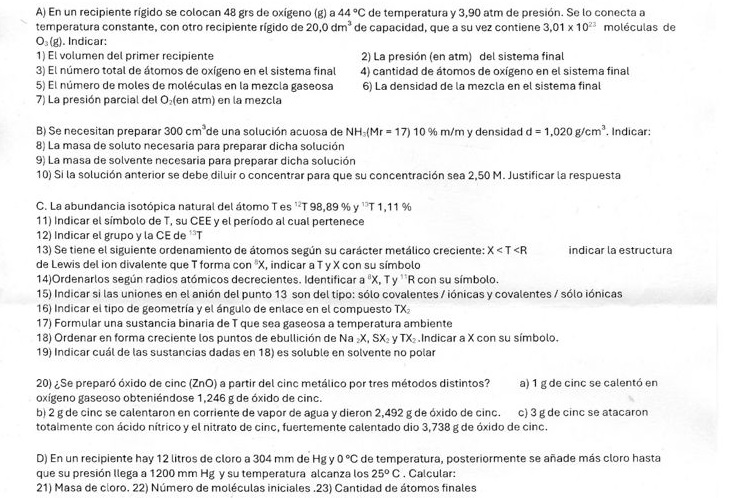
\includegraphics[width=0.7\linewidth]{Images/molinos_examen_6.jpg}
\end{figure}


\subsection*{Resolución}

\begin{enumerate}[left=0cm]
\setlength\itemsep{2\baselineskip}

\item ¿Volumen del primer recipiente?

Datos:

\hfil48g de \ce{O2} $\equiv$ 1,5 mol\hfil 44ºC = 317 K\hfil 3,9 atm\hfil

Uso ecuación de gases ideales:
\begin{align*}
    P\cdot V &= n \cdot R \cdot T\\
    3,9 \text{atm}\cdot V &= 1,5\text{mol} \cdot 0,082\dfrac{\text{atm}\cdot \text{L}}{\text{mol}\cdot\text{K}}  \cdot 317 \text{K}\\
    V &= 10 \text{ L}
\end{align*}


\item ¿Presión del sistema final?

\hfil
$V_{\text{Total}} = 10 \text{L} + 20 \text{L}$
\hfil
$n_{\text{Total}} = 0,5 \text{mol} + 1,5 \text{mol}$
\hfil
T = 317 K
\hfil

Uso ecuación de gases ideales:
\begin{align*}
    P\cdot V &= n \cdot R \cdot T\\
    P\cdot 30 \text{L} &= 2\text{mol} \cdot 0,082\dfrac{\text{atm}\cdot \text{L}}{\text{mol}\cdot\text{K}}  \cdot 317 \text{K}\\
    P &= 1,73 \text{ atm}
\end{align*}


\item ¿Número de átomos de oxígeno en el sistema final?

Hay 1,5 mol de \ce{O2} y 0,5 mol de \ce{O3}. Del gas oxígeno tengo 3 moles de átomos de O y del ozono tengo 1,5 mol de O.

$$n = 4,5 \cdot 6,02 \cdot 10^{23} = 2,71 \cdot 10^{24}$$


\item ¿Cantidad de átomos de oxígeno en el sistema final?

Pregunta lo mismo que en el punto anterior.


\item ¿Número de moles de moléculas en la mezcla gaseosa?

$$n = 1,5 \text{mol} + 0,5 \text{mol} = 2 \text{mol}$$


\item ¿Densidad de la mezcla final?

\hfil
48g de \ce{O2}
\hfil
0,5 mol de \ce{O3} $\equiv$ 24g de \ce{O3}
\hfil

$$\delta = \dfrac{72 \text{g}}{30 \text{L}} = 2,4 \dfrac{\text{g}}{\text{L}}$$


\item ¿Presión parcial del \ce{O2} en la mezcla?

\hfil
1,5 mol de \ce{O2}
\hfil
$V = 30$L 
\hfil
$T=317$ K
\hfil

Uso ecuación de gases ideales:
\begin{align*}
    P\cdot V &= n \cdot R \cdot T\\
    P_{\ce{O2}} \cdot 30 \text{L} &= 1,5\text{mol} \cdot 0,082\dfrac{\text{atm}\cdot \text{L}}{\text{mol}\cdot\text{K}}  \cdot 317 \text{K}\\
    P_{\ce{O2}} &= 1,30 \text{ atm}
\end{align*}


\item Indicar la masa de soluto:

\hfil
300 ml de SC \hfil
ST es \ce{NH3} \hfil 
10\%m/m\hfil
$\delta$=1,02 g/cm${^3}$ 
\hfil

Hay 306 g de SC, entonces habrán 30,6 g de \ce{NH3}


\item Masa de solvente necesaria para preparar dicha solución:

\hfil$306\text{ g} - 30,6\text{ g} = 275,4\text{ g}$\hfil

\item Si la solución anterior se debe diluir o concentrar para que su concentración sea 2,5 M. Justificar la respuesta.

\end{enumerate}
